\documentclass[thesis]{subfiles}

\begin{document}

\chapter{Foundations}
\label{chapter:foundations}

% TODO: Reference the checklist from the previous chapter

% NOTE: This is sooo hard to write well.
\pyop3 was created to be a successor to \pyop2, and so it is instructive to review how \pyop2 works and identify any shortcomings.
We will then review a number of libraries whose abstractions capture the missing behaviour.

\section{\pyop2}
% NOTE: should mention partial GPU support (cite Kaushik)
% NOTE: should mention extruded (then mention at end of doc)

Just like \pyop3, \pyop2 is an execution model for the application of compact computational kernels over unstructured meshes~\cite{rathgeberPyOP2HighLevelFramework2012}.
It was introduced to provide the same abstractions as OP2~\cite{mudaligeOP2ActiveLibrary2012} but using runtime code generation instead of source-to-source translation.
It is a core component of the Firedrake finite element framework~\cite{FiredrakeUserManual}.

\subsection{Data structures}

\pyop2 has no innate concept of what an unstructured mesh is.
Instead, topological entities are treated as \textit{sets}, with \textit{mappings} between the different sets.

There are 3 different types of data structures defined in \pyop2: globally constant values, vectors and matrices.
These are termed \pycode{Globals}, \pycode{Dats} and \pycode{Mats} respectively.

For more complex problems like the Stokes equations in \cref{sec:stokes_equations} the \glspl{dof} are associated with multiple types of topological entity.
In \cref{fig:scott_vogelius_element_P3} for example the unknowns are associated with the cell, edges and vertices.
This means that one has to associate the \glspl{dof} for that function space with a distinct \textit{node set}, rather than a set for a particular topological entity.
As a consequence, the data structures do not know to what topological entity they refer and the library user must take responsibility for constructing the right maps from, say, cells to nodes.

\subsection{Loops}

In order to apply kernels to these data structures, a \textit{parallel loop} (\pycode{par_loop}) is constructed and executed.
The loop takes as arguments a \textit{local kernel}, \textit{iteration set} and zero or more \textit{arguments} that provide the data structures needed by the local kernel.

% mention loopy here briefly (cref{sec:pyop2_codegen})

% arguments may need map from iteration set to its own (node) set, also accessors


An example loop statement is shown in \cref{fig:pyop2_parloop}.

\subsection{Code generation}
\label{sec:pyop2_codegen}

\begin{figure}
  \includegraphics{pyop2_codegen_flowchart.pdf}
  \caption{Simplified code generation pathway for a \pyop2 parallel loop.}
  \label{fig:pyop2_codegen}
\end{figure}

\begin{figure}
  \centering
  \begin{subfigure}{.49\textwidth}
    \begin{pylisting}
      knl = loopy.make_kernel(
        "{ [i]: 0 <= i < n }",  # domains
        "y[i] = 2*x[i]",        # instructions
        [                       # arguments
          loopy.GlobalArg("x", dtype=float),
          loopy.GlobalArg("y", dtype=float),
          loopy.ValueArg("n", dtype=int),
        ],
      )
    \end{pylisting}
    \caption{Python code to construct the kernel. Some arguments to \pycode{make_kernel} have been omitted for simplicity.}
    \label{fig:loopy_codegen_kernel}
  \end{subfigure}
  %
  \begin{subfigure}{.49\textwidth}
    \inputminted[fontsize=\footnotesize]{c}{./scripts/artefacts/loopy_example_c_code_tidy.c}
    \caption{The generated C code.}
    \label{fig:loopy_codegen_c}
  \end{subfigure}

  \caption{
    An example loopy kernel.
    The kernel takes two array arguments, \pycode{x} and \pycode{y}, and sets the values in \pycode{y} to twice those in \pycode{x}.
    Both arrays have the same unknown length \pycode{n} which is also passed in to the kernel as an argument.
  }
  \label{fig:loopy_codegen}
\end{figure}

The code generation pipeline is summarised in \cref{fig:pyop2_codegen}.
Having constructed a parallel loop, \pyop2 executes it by first lowering the loop object through a sequence of intermediate representations before compiling and running the generated low-level code.

The first intermediate representation is loopy~\cite{klocknerLooPyTransformationbased2014}, a polyhedral model inspired Python code generation library.

With loopy, the main entry point is the declaration of a \pycode{LoopKernel}.
To construct such a kernel, the user needs to specify \textit{domains}, \textit{instructions} and \textit{arguments}.
An example loopy kernel is shown in \cref{fig:loopy_codegen_kernel}, with the generated C string shown in \cref{fig:loopy_codegen_c}.

% TODO: talk about GPUs
loopy is capable of generating code for multiple backends including CPUs and GPUs and so \pyop2 targeting loopy should, in principle, allow the same \pyop2 code to target different architectures.

% TODO: talk about vectorisation (cite TJ)
Once a \pycode{LoopKernel} has been created, loopy also provides a wealth of different code transformations such as loop tiling, vectorisation and loop-invariant code motion.

\subsection{Parallel execution}
\label{sec:pyop2_parallel}

% NOTE: I am deciding to not try too hard to explain core/owned/ghost because I
% think that the design is poor and I demonstrate something better later.

\begin{algorithm}
  \begin{verbatim}
Trigger required halo exchanges
FOR EACH item IN iterset.core:
  compute(item)

Await halo exchanges
FOR EACH item IN iterset.owned:
  compute(item)
  \end{verbatim}
  \caption{The \pyop2 parallel loop execution algorithm to interleave computation and communication.}
  \label{alg:pyop2_comp_comm_overlap}
\end{algorithm}

By keeping careful track of the parallel decomposition of sets, \pyop2 is capable of interleaving computation and communication when executing parallel loops.
To do so each set is split into 3 parts:

\begin{itemize}
  \item \textit{Core}: Set elements that do not require any data from other processes during a parallel loop.

  \item \textit{Owned}: Set elements that belong to the current process but do require data from other processes.

  \item \textit{Ghost}: Set elements present on a process that belong to another process.
\end{itemize}

  % Given this partitioning, \pyop2 then reorders the data such that it looks like:
  %
  % \begin{center}
  %   \includegraphics{pyop2_partition.pdf}
  % \end{center}

% NOTE: closure is a new term here
The number of \textit{ghost} points is known to the mesh already, as it has knowledge of its overlap.
To determine the \textit{core} and \textit{owned} partitions one loops over the cells of a mesh and inspecting all the points in the closure of the cell.
If any of the points in the closure are \textit{ghost}, then all other points in the closure are marked as \textit{owned}.
Any remaining points without a label are labelled \textit{core}.

From this partitioning it is possible to interleave computation and communication.
Computations over points marked \textit{core} are not influenced by any ghost data and so can proceed before ghost data has been communicated. \textit{Owned} points need to have up-to-date ghost data and so must wait for all communication to be completed before beginning.
This is shown in \cref{alg:pyop2_comp_comm_overlap}.

% NOTE: This is an acceptable repeat of the sorts of things said in chapter 1.
\subsection{Limitations}

% NOTE: Not sure I have anything to actually ref here
As mentioned in \cref{sec:???}, \pyop2 is negatively affected by a number of design choices that limit its suitability:

% NOTE: bad spacing
\paragraph{Poor composability}{
  Associating mesh data with \textit{node sets} discards topological information and places a burden on the library user to keep track of the relations between the mesh topology and the nodes.
}

\paragraph{Inflexible interface}{
  Not all mesh operations are expressible as a single kernel executed within a single loop over entities.
  Algorithms for physics-based preconditioners such as hybridisation~\cite{gibsonSlateExtendingFiredrake2020} and additive Schwartz methods~\cite{farrellPCPATCHSoftwareTopological2021} involve multiple kernels and nested loops and so implementing them required sui-generis additions to \pyop2 that are difficult to extend.
  It would be preferable to have an abstraction for mesh computations that was sufficiently flexible for these algorithms to be expressible.
}

\pyop3 aims to resolve both of these limitations with \pyop2 by rethinking the core abstractions.
The design of a number of libraries were used as inspiration for approaches to solving these problems.
These will be reviewed below.

\section{Relating unknowns to mesh topology: DMPlex}
\label{sec:foundations_dmplex}

% NOTE: Where is PETSc first mentioned? Possibly here is a good place for more detail about it.
% Should be mentioned in the introduction
To tackle the problem of composability - sets discarding information about mesh topology - we look to DMPlex~\cite{knepleyMeshAlgorithmsPDE2009,langeEfficientMeshManagement2016,knepleyUnstructuredOverlappingMesh2015}.
DMPlex is an abstraction for unstructured meshes bundled with PETSc, a scientific software toolkit providing implementations of parallel vectors and matrices as well as a plethora of linear and non-linear solvers~\cite{petsc-web-page,petsc-user-ref,petsc-efficient}.
It has support for a range of complex mesh operations such as mesh refinement, I/O~\cite{hamEfficientNtoMCheckpointing2024}, all in parallel (\cref{sec:dmplex_parallel}).  % TODO: needs more...

\begin{figure}
  \centering
  \begin{subfigure}{.49\textwidth}
    \centering
    \includegraphics{two_cell_mesh.pdf}
  \end{subfigure}
  %
  \begin{subfigure}{.49\textwidth}
    \centering
    \includegraphics{dmplex_hasse.pdf}
  \end{subfigure}
  \caption{TODO, mention Hasse diagram}
  \label{fig:dmplex_hasse}
\end{figure}

With DMPlex, the unstructured mesh is represented as a \gls{dag} (\cref{fig:dmplex_hasse}).
All topological entities are referred to as \textit{points}, with each entity type belonging to a particular \textit{strata} of the overall \gls{dag}.
\textit{Arrows} connect points between strata to represent the connectivity of the different entities.
For example every edge in a mesh (depth 1) has two arrows pointing at its two \textit{covered} vertices (depth 0).
By treating all entities as points, DMPlex is capable of expressing unstructured meshes of any dimension.

\begin{figure}
  \centering
  \begin{subfigure}{.49\textwidth}
    \centering
    \includegraphics{dmplex_hasse_cone.pdf}
    \caption{$\cone(0) = \{6,7,8\}$}
  \end{subfigure}
  %
  \begin{subfigure}{.49\textwidth}
    \centering
    \includegraphics{dmplex_hasse_support.pdf}
    \caption{$\support(8) = \{0,1\}$}
  \end{subfigure}

  \begin{subfigure}{.49\textwidth}
    \centering
    \includegraphics{dmplex_hasse_closure.pdf}
    \caption{$\closure(0) = \{0,6,7,8,2,3,4\}$}
  \end{subfigure}
  %
  \begin{subfigure}{.49\textwidth}
    \centering
    \includegraphics{dmplex_hasse_star.pdf}
    \caption{$\plexstar(3) = \{3,7,8,9,0,1\}$}
  \end{subfigure}

  \caption{
    The possible DMPlex covering queries applied to the Hasse diagram from Figure~\ref{fig:dmplex_hasse}.
  }
  \label{fig:dmplex_queries}
\end{figure}

DMPlex has a simple query language that can be used to traverse the \gls{dag} and build appropriate stencils.
It consists of two core operations: \textit{cone} and \textit{support}.
The cone of a point, written $\cone(p)$, is the set of points that are pointed to from $p$.
The support of a point, written $\support(p)$, is the dual of cone and yields the set of points that point to $p$.
Transitive closures for both of these operations, where the operation is applied repeatedly and all points are accumulated, are also supplied by DMPlex.
The transitive closure of cone is termed the \textit{closure} ($\closure(p)$) and the transitive closure of support is called the \textit{star} ($\plexstar(p)$).
These operations are shown in \cref{fig:dmplex_queries}.

It is possible to compose these operations to yield larger stencils.
For instance $\support(\cone(p))$ with $p$ a cell produces the set of cells sharing an edge with $p$ (and $p$ itself).
Likewise, $\closure(\star(p))$ is the \textit{adjacency} relation for finite element calculations: basis functions on points within this stencil have non-zero support with the basis functions on $p$.

\subsection{Representing data layouts}
\label{sec:dmplex_data_layout}

\begin{figure}
  \begin{clisting}
    // set cell DoFs
    DMPlexGetDepthStratum(dmplex, 2, &start, &end);
    for (int cell=start; cell<end; cell++)
      PetscSectionSetDof(section, cell, 2);

    // set edge DoFs
    DMPlexGetDepthStratum(dmplex, 1, &start, &end);
    for (int edge=start; edge<end; edge++)
      PetscSectionSetDof(section, edge, 4);

    # set vertex DoFs
    DMPlexGetDepthStratum(dmplex, 0, &start, &end);
    for (int vertex=start; vertex<end; vertex++)
      PetscSectionSetDof(section, vertex, 2);

    PetscSectionSetUp(section);
  \end{clisting}

  \caption{
    C code constructing an appropriate \ccode{Section} for a $[P_3]^2$ finite element (\cref{fig:scott_vogelius_element_P3}).
    Some boilerplate code is omitted.
  }
  \label{fig:section_p3}
\end{figure}

\begin{algorithm}
  \begin{verbatim}
counter = 0
offset = 0
FOR EACH point IN chart
  renumbered_point = renumber(point)
  offsets[counter] = offset
  counter += 1
  offset += PetscSectionGetDof(renumbered_point)
  \end{verbatim}

  \caption{
    The tabulation algorithm that determines the right offsets from a \ccode{Section}.
    This code is executed during \ccode{PetscSectionSetUp()}.
  }
  \label{alg:petsc_section_tabulate}
\end{algorithm}

In order to associate data with these mesh points, a user typical constructs a \ccode{Section} object.
These are simple CSR-like data structures that associate mesh points with offsets into an array.

\ccode{Sections} are constructed by assigning a number of \glspl{dof} with each mesh point (\cref{fig:section_p3}).
Once the number of \glspl{dof} has been specified, calling \ccode{PetscSectionSetUp()} traverses the input points and accumulates the offset for each point.
As a simple example, given the \gls{dof} count \ccode{[1, 0, 3, 2, 0, 1]} the \ccode{Section} would tabulate the following offsets: \ccode{[0, 1, 1, 4, 6, 6]} (\cref{alg:petsc_section_tabulate}).

\ccode{Sections} are also able to express the sorts of renumbering locality optimisations described in \cref{sec:intro_mesh_numbering}.
One simply provides the \ccode{Section} with a \textit{permutation} that is accounted for during set up (\cref{alg:petsc_section_tabulate}).

Whilst a powerful tool for describing data layouts, \ccode{Sections} have a number of limitations:

\begin{itemize}
  \item
    \textbf{They are fully ragged}\\
    \ccode{Sections} do not distinguish between different types of topological entity and so important structure cannot be represented.
    They only store DoF information per point in a completely unstructured way and are incapable of knowing, say, that every cell in the mesh stores exactly one DoF.
    This can prohibit the compiler from making certain optimisations (e.g. loop unrolling) that it would have been able to do were it to know of a constant loop extent.
    Additionally, this variable size increases memory pressure as redundant arrays of constant sizes need to be streamed through memory.

  \item
    \textbf{Shape information is lost}\\
    Though \ccode{Sections} allow one to directly associate \glspl{dof} with mesh entities of different dimension, they still lose information about the structure of the function space.
    For instance, to a \ccode{Section}, a point with a single vector-valued node is indistinguishable from a point with multiple nodes.
\end{itemize}

These limitations prevent \pyop3 from directly using \ccode{Sections} to describe its data layouts, but it takes a similar approach:

\begin{itemize}
  \item All topological entities in the mesh should be equivalent,
  \item Interleaved points require one to tabulate an array of offsets (\cref{alg:petsc_section_tabulate}).
\end{itemize}

\subsection{Parallel}
\label{sec:dmplex_parallel}

As touched upon in \cref{sec:intro_mpi}, DMPlex works in parallel by partitioning the entire ``global" mesh into local pieces that are kept on each process.
Each local piece of the mesh is \textit{closed}, meaning that all points in the cell closures are represented locally.
This means that there are \textit{ghost} points kept on each process that are owned by other processes.

\subsubsection{Star forests}

\begin{figure}
  \centering
  %
  \begin{subfigure}{\textwidth}
    \centering
    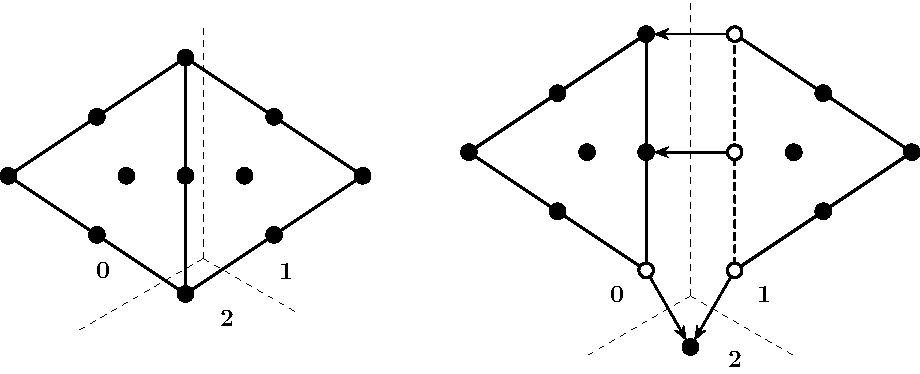
\includegraphics{star_forest_point.pdf}
    \caption{TODO}
    \label{fig:star_forest_point}
  \end{subfigure}
  %
  \begin{subfigure}{\textwidth}
    \centering
    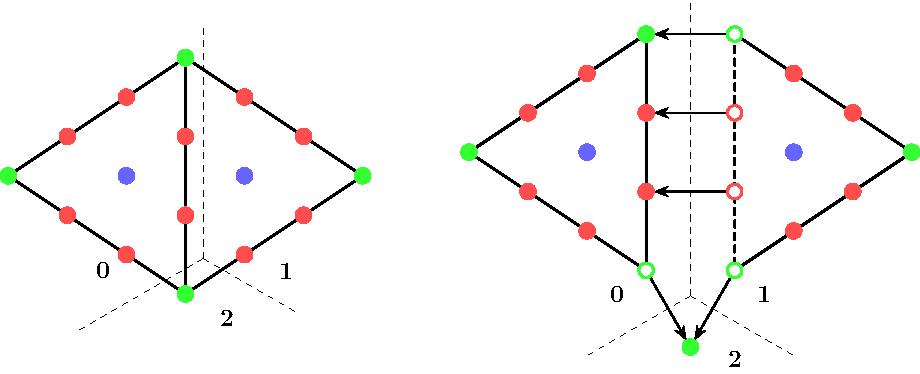
\includegraphics{star_forest_dof.pdf}
    \caption{TODO}
    \label{fig:star_forest_dof}
  \end{subfigure}
  %
  \caption{TODO}
  \label{fig:star_forest}
\end{figure}

\begin{figure}
  \centering
  \begin{subfigure}{.6\textwidth}
    \centering
    \includegraphics{star_forest_abstract_mesh.pdf}
    \caption{Star forest suitable for describing the point sharing in \cref{fig:star_forest_point}.}
  \end{subfigure}
  %
  \begin{subfigure}{.39\textwidth}
    \centering
    \includegraphics{star_forest_abstract_global.pdf}
    \caption{Star forest appropriate for storing the communication pattern of a globally consistent value.}
  \end{subfigure}
  \caption{
    Common star forest patterns.
    Each point is labelled with its owning process and root and leaf points are shown in black and white respectively.
  }
  \label{fig:star_forest_abstract}
\end{figure}

% supports broadcasts from the root and reductions from the leaves

Parallel communication in DMPlex is handled by \textit{star forest} objects (\ccode{PetscSF}) \parencite{zhangPetscSFScalableCommunication2021}.
Star forests relate equivalent points across processes as a collection - or ``forest" - of ``stars".
A ``star" is a directed graph with depth 1 and a single root.

Star forests are effective for describing point-to-point MPI operations because they naturally encode the source and destination nodes as roots and leaves of the stars.
They can flexibly describe a range of different communication patterns.
For example, a value shared globally across $n$ ranks can be represented as a star forest containing a single star with the root node on rank 0 and $n-1$ leaves, 1 for each other rank.
This is shown in Figure~\ref{fig:???}.
Star forests are also suitable for describing the overlap between parts of a distributed mesh.
In this case, each star in the forest represents a single point (cell, edge, vertex) in the mesh with the root on the ``owning" rank and leaves on the ranks where the point appears as a ``ghost".
An example of such a distribution is shown in Figure~\ref{???}.

% Because local numbers on one process are related to local numbers on other processes no global enumeration of points is strictly required.

Upon construction a DMPlex holds a \textit{point star forest} that stores the information about ghost points (\cref{fig:star_forest_point}).
This is insufficient for function data to be communicated correctly though because the number of \glspl{dof} associated with each entity can change.
To transfer function data, PETSc composes the point star forest with a \ccode{Section} to produce a new star forest (\cref{fig:star_forest_dof}).

% maybe use alg. from chapter 6 here?

        % def create_dof_sf_inner(axis: Axis, component: AxisComponent, ...):
        %   section = create_section(axis, component)
        %   dof_sf = component.sf.createSectionSF(section, ...)
        %   return dof_sf

\section{A language for structured data: numpy}

numpy is ...

numpy has established itself as the de-facto approach for high level libraries to...

Much of the following thesis can be viewed as a generalisation of numpy-like abstractions, and so it is useful to establish the relevant terminology now.

% (cite paper, search for "citing numpy")
% although not a JIT, numpy is important for introducing ergonomic ways of
% expressing array computations
% there are some numpy JIT options out there: JAX, pytato, pytorch?

\subsection{N-dimensional arrays}

The key abstraction introduced by numpy is the \textit{N-dimensional array}, or \pycode{ndarray}.
It is an intuitive and widely used interface for operating on multi-dimensional data.

% not suitable for pyop3 because we have more heterogeneous data layouts (but works for pyop2 node sets)

% shape
% broadcast/vectorised operations

% implemented as a header and a buffer
% stride information (for views)

\subsection{Indexing arrays}
\label{sec:numpy_indexing_arrays}

\begin{table}
  \centering

  \begin{tabular}{|l|l|l|l|}
    \hline
    \textbf{Index operation} & \textbf{Example} & \textbf{Return value} & \textbf{Array return type} \\
    \hline
    Single element indexing & \pycode{array[1]} & \pycode{"B"} & N/A \\
    \hline
    Slicing & \pycode{array[1:6:2]} & \pycode{["B", "D", "F"]} & View \\
    \hline
    Integer array indexing & \pycode{array[[0, 3, 4]]} & \pycode{["A", "D", "E"]} & Copy \\
    \hline
  \end{tabular}

  \caption{
    Common indexing operations for numpy arrays.
    The examples shown apply the index to the string array \pycode{["A", "B", "C", "D", "E", "F"]} (called \pycode{array} above).
    The array return type for single element indexing is marked as ``N/A" because a string is returned instead of an array.
  }
  \label{tab:numpy_indexing_ops}
\end{table}

Broadcasting operations, that handle the entire array monolithically, are not adequate for many programs.
numpy, therefore, allows for array \textit{indexing}, where portions of the full array are extracted to yield a new array.

Some of the ways that a numpy array may be indexed are shown in \cref{tab:numpy_indexing_ops}:

\begin{itemize}
  \item \textbf{Single element indexing}

    Single element indexing takes an integer and simply returns the value stored at that point.

  \item \textbf{Slicing}

    Slices are a standard Python concept for describing ranges of indices and have the syntax \pycode{[start:stop:step]}.
    Omitting \pycode{start}, \pycode{stop} or \pycode{step} will default to 0, the end of the array, and 1 respectively.
    In the example shown in \cref{tab:numpy_indexing_ops} the slice \pycode{[1:6:2]} corresponds to asking for ``the values in the array from index 1 (inclusive) to index 6 (exclusive), striding by 2".

  \item \textbf{Integer array indexing}

    Integer array indexing returns a new array containing values stored at the requested indices, for the example in \cref{tab:numpy_indexing_ops} this simply being 0, 3 and 4.

\end{itemize}

% These operations work together with the header specs to figure out the right offsets.

Although the examples provided are all for a 1-dimensional array, it is completely permissible to index N-dimensional arrays with a collection of these indexing operations, one per axis of the array.
This collection of indices is termed a \textit{multi-index}.

numpy draws a distinction between ``basic" indexing, single element indexing and slicing, and ``advanced" indexing like using integer arrays.
For the former, the array returned from the indexing operation is a \textit{view}, whereas for the latter a \textit{copy} is returned.
Alongside the obvious memory advantages, views are also preferable to copies because they are \textit{composable}.
One can take views of views repeatedly without triggering a copy, allowing for changes to the indexed array to be propagated back to the original.

% mention in chapter 4!
% In \pyop3, as well as generalising the indexing operations above to axis trees, we overcome this shortcoming of numpy's advanced indexing such that views are always used regardless of the indexing method used.

\end{document}
